% !TeX spellcheck = de_DE
\rhead{28 Mai 2018}

\section{Henselsche Körper}

\begin{erinnerung*}[Theorem 4, Lemma von Hensel]
	Sei $K$ ein vollständiger Körper. Seien $f \in \O[X]$ ein primitives Polynom,
	\[\proj: \O[X] \to \kappa[X]\]
	die natürliche Projektion und $\bar{f}=\proj(f)$. Falls $\bar{f}=\bar{g}\bar{h}$ mit $\bar{g}, \bar{h} \in \kappa[X]$ teilerfremd, dann gibt es $g,h \in \O[X]$ mit:
	\begin{enumerate}[(i)]
		\item $f(X)=g(X)h(X)$
		\item $\proj(g)=\bar{g}$ und $\proj(h)=\bar{h}$
		\item $\deg(g)=\deg(\bar{g})$
	\end{enumerate}
\end{erinnerung*}

\begin{Bsp*}
	Haben $X^2+7$ bzw. $X^2+6$ Lösungen über $\Q_5$. Wegen $X^2 -7 = X^2 -2$ und $X^2 \neq 2$ für alle $X=1,2,3,4$ hat erste Gleichung keine Lösung in $\Z_5$.
	Wegen
	\[ X^2-6 =X^2-1=(X-1)(X+1)
	\]
	in $\Z_5$ existiert nach Hensel auch eine Lösung in $\Q_5$.
	
	Insbesondere folgt aus erstem Beispiel, dass $\Q_5$ nicht algebraisch abgeschlossen ist.
\end{Bsp*}


\begin{defi}
	Ein Körper $K$ mit Bewertung $v$, der die Aussage vom Lemma von Hensel (Theorem 4) erfüllt, heißt \textbf{Henselscher Körper}.
\end{defi}

\begin{Bsp}
	Sei $\Q_p^{\alg} = \{ \alpha \in \Q_p; \, \alpha \text{ algebraisch über } \Q  \}$.
	Dann ist $\Q_p^{\alg}$ ein Henselscher Körper.
\end{Bsp}

\begin{proof}
	Sei $\hat{\O}^{\alg}$ der Bewertungsring in $\Q_p^{\alg}$ und $f\in\hat{\O}^{\alg}[X]$
	mit $f$ primitiv und $\overline{f} = \overline{g} \overline{h}$ in $\F_p[X]$ mit $\overline{g}, \overline{h}$ teilerfremd.
	Nach Hensels Lemma gibt es $g,h \in \O[X]$ mit $f=gh$ und $\deg g = \deg \overline{g}$ so, dass $\overline{g}$ und $\overline{h}$ jeweils die Bilder von $g$ und $h$ in $\F_p[X]$ sind. Hierbei sei $\O$ der Bewertungsring von $\Q_p$.
	
	\bigskip Sei $\overline{\Q}$ der algebraische Abschluss von $\Q$. Setze $v_p$ und $\abs{\cdot}_p$ auf $\overline{\Q}$ fort. Sei $\hat{\overline{\Q}}$ die metrische Komplettierung von $\overline{\Q}$. Erhalte folgendes Diagramm:
	\[ \begin{tikzcd}
	\Q_p
	\arrow[hookrightarrow]{r}
	& \hat{\overline{\Q}}
	\\
	\Q
	\arrow[hookrightarrow]{r}
	\arrow[hookrightarrow]{u}
	&\overline{\Q}
	\arrow[hookrightarrow]{u}
	\\
	\end{tikzcd}
	\]
Über $\overline{\Q}$ zerfällt $f$ in Linearfaktoren $f=(X-\alpha_1) \cdots (X-\alpha_n)$ mit $\alpha_1, \dots, \alpha_n \in\overline{\Q}$. Nach Umsortieren können wir also annehmen, dass
$g=(X-\alpha_1) \cdots (X-\alpha_r)$ und $h=(X-\alpha_{r+1}) \cdots (X-\alpha_n)$ . Also liegen die Koeffizienten von $g$ und $h$ in $\overline{\Q} \cap \Q_p = \Q_p^{\alg}$ so, dass $g,h \in \Q_p^{\alg}[X]$. Somit ist Hensels Lemma erfüllt.
\end{proof}

\begin{Prop}
	Seien $(K,v)$ ein Henselscher Körper und $L/K$ eine algebraische Erweiterung. Dann hat $v$ auf $L$ eine eindeutige Fortsetzung $w$ und der Bewertungsring $\O_w$ von $w$ is der ganze Abschluss vom Bewertungsring $\O_v$ von $v$. Ist $L/K$ endlich vom Grad $n$, dann ist $w$ gegeben durch
	\[ w(\alpha) = \frac{1}{n} v \left( \Norm_{L/K} ( \alpha) \right)
	\]
	und
	\[ \abs{\alpha} = \sqrt[n]{\abs{\Norm_{L/K}(\alpha)}}.
	\]
\end{Prop}


\begin{Bem}[\enquote{Knackpunkt}]
	Sei $(K,v)$ Henselsch mit Bewertungsring $\O_v$ und maximalem Ideal $\p_v$.
	Sei $f= a_nX^n + \cdots + a_0 \in K[X]$ irreduzibel. Dann gilt
	\[ \abs{f} =\max \{  \abs{a_0}, \dots, \abs{a_n} \}.
	\]
\end{Bem}

\begin{proof}
	Wie in Korollar 5.6.5.
\end{proof}

\begin{proof}[Proof (Proposition 5.8.3)]
	Wie in Theorem 5.
\end{proof}

Als nächstes wollen wir zeigen, dass in Proposition 5.8.3 auch die umgekehrte Implikation gilt.
Dazu wollen wir erst Folgendes zeigen:

\bigskip Wenn $v$ von $K$ auf einem Zerfällungskörper $Z(f)$ für ein $f\in K[X]$ fortgesetzt werden kann, dann \enquote{kennen} die Bewertungen der Koeffizienten von $f$ schon die Bewertungen der Nullstellen von $f$.

\begin{Bsp}
	\textbf{(1)} Seien $p=3$, $v= v_3$ und
	\begin{align*}
	h(X)
	&= X^7-6x^6-55X^5+222X^4 +459X^3-1674X^2-405X+1458 \\
	&=(X-1)(X+1)(X+3)(X-3)^2(X+6)(X-9).
	\end{align*}
	Es ist
	\begin{align*}
	v(1)=v(-1)&=0, \\
	v(3)=v(-3)=v(6)&=1, \\
	v(9)&=2.
	\end{align*}
	
	\bigskip \textbf{(2)} Zeichne einen Streckenzug durch die Punkte $(i,v(a_i))$ 
	und die untere konvexe Einhüllende $H$ davon. Der untere Rand von $H$ heißt Newton-Polygon. Dieser besteht aus den drei Kanten $e_1, e_2, e_3$.
	\begin{center}
		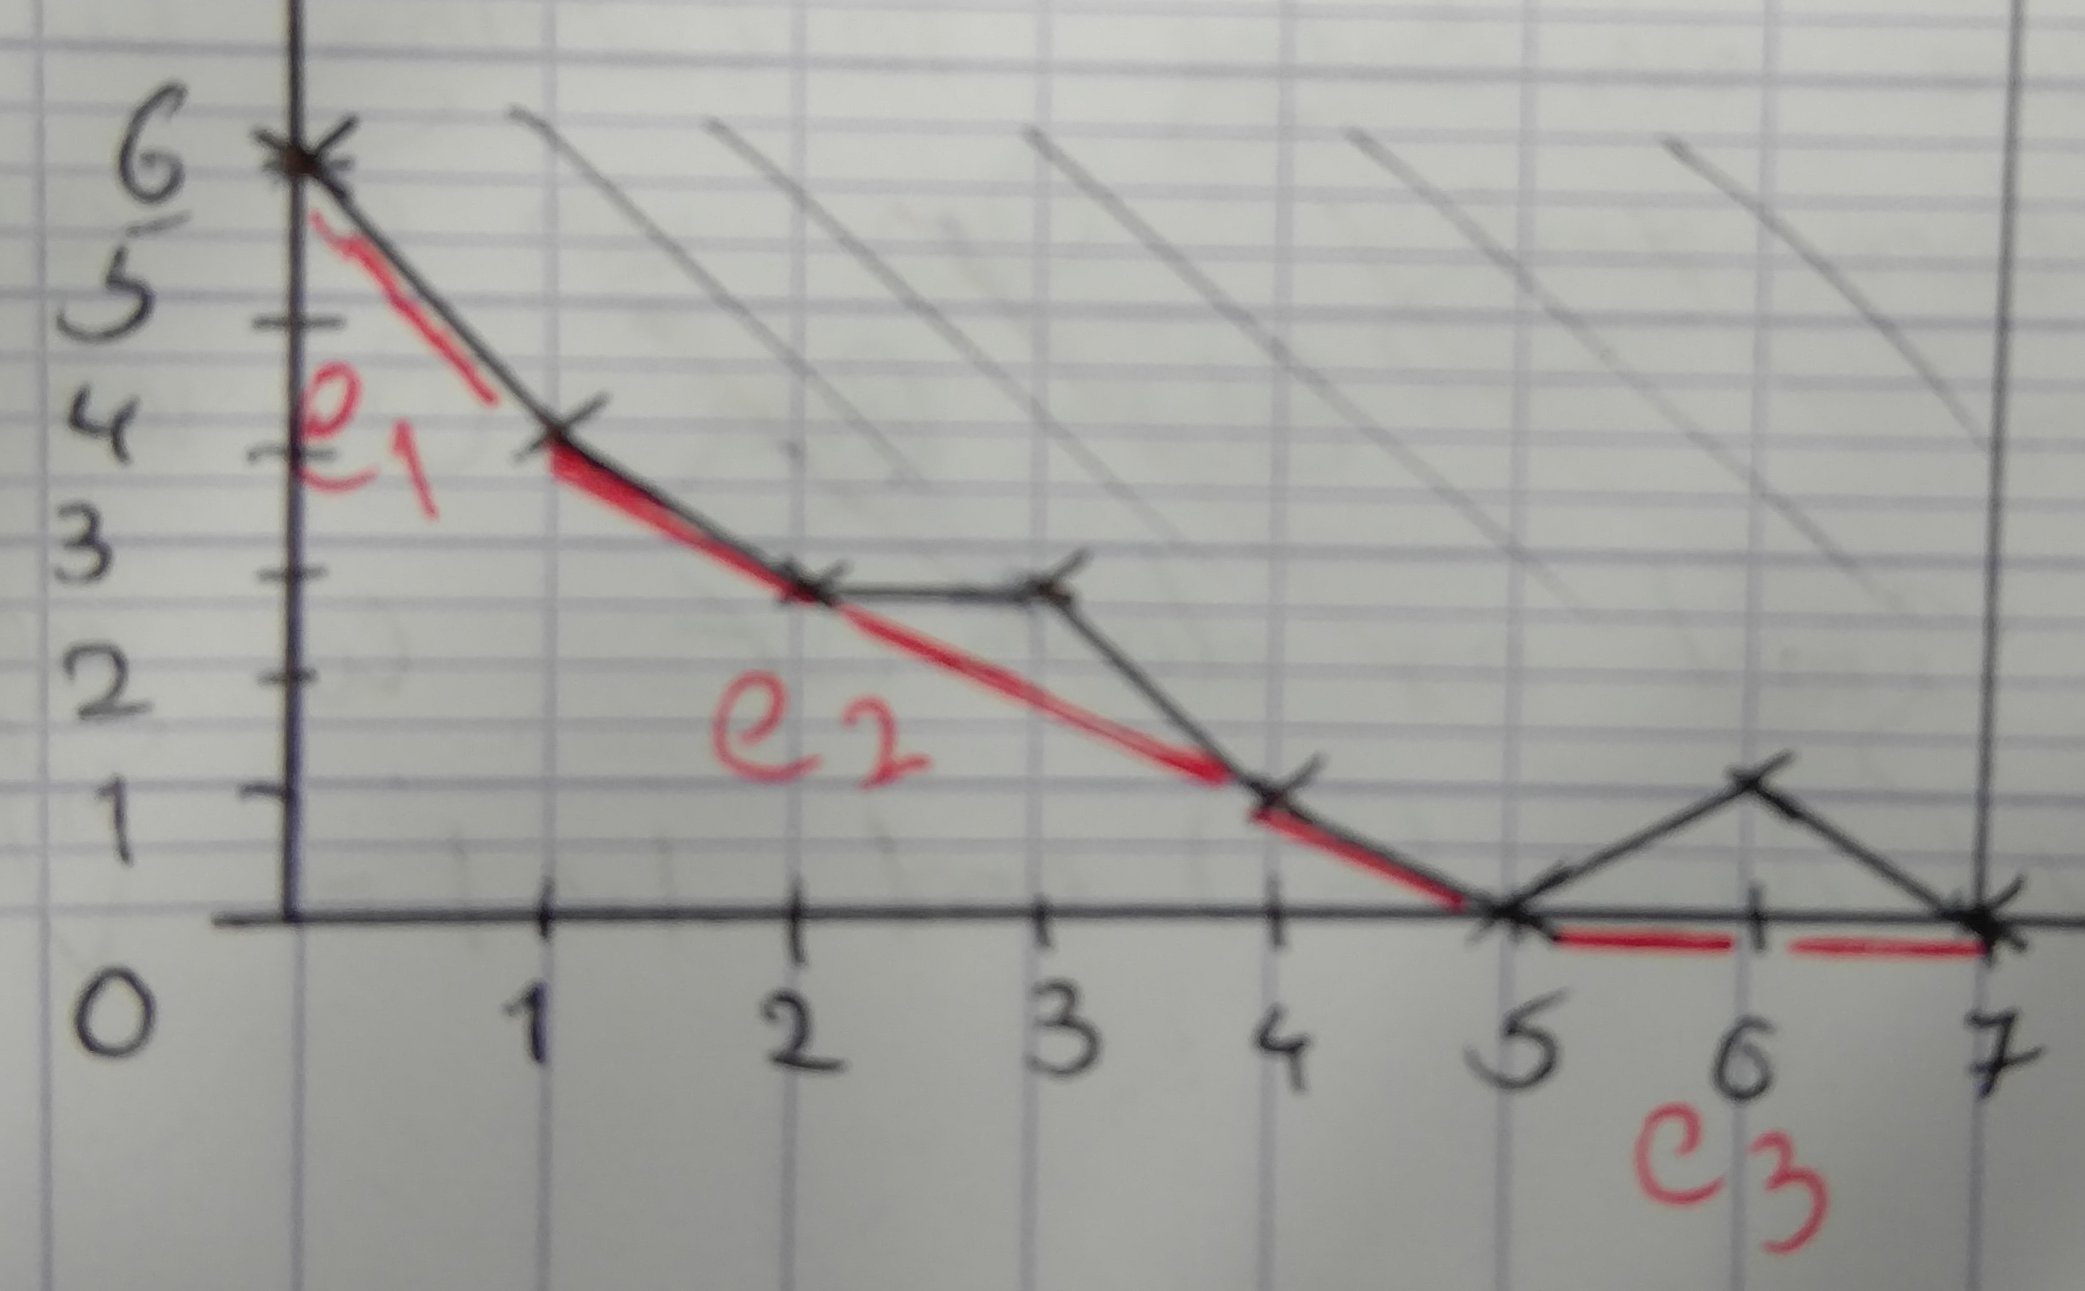
\includegraphics[width=0.4\textwidth]{img/newton_polynomial.png}
	\end{center}
	
	\bigskip \textbf{(3)} Ordne den $3$ Kanten  $e_1, e_2, e_3$ jeweils ihre Steigung $m_1=-2$, $m_2 = -1$ und $m_3=0$ sowie ihre kombinatorische Länge $c_1 = 1$, $c_2 =4$ und $c_3 = 2$ zu.
	
	\bigskip \textbf{(4)} Beobachtung: $h$ hat $c_i$ Nullstellen $\alpha$ mit Bewertung $v(\alpha) = -m_i$.
\end{Bsp}

\begin{defi}
	Seien $K$ ein Körper mit Bewertung $v$ und $f(X)=a_nX^n+ \cdots + a_0 \in K[X]$ mit $a_n a_0 \neq 0$. Sei
	\[ I = \left\{
		i \in \{ 0, \dots, n \}; \, a_i \neq 0
	\right\}
	\]
	und sei $H$ die untere Einhüllende der Punktemenge $\{ (i,v(a_i)); \, i \in I  \}$. Dann wird $H$ nach unten beschränkt durch einen Kantenzug $(e_1, \dots, e_k)$ mit Startpunkt $(0,v(a_0))$ und Endpunkt $(n,v(a_n))$. Dieser Streckenzug heißt \textbf{Newton-Polygon} von $f$.
	Jeder Strecke $e_i$ ordnen wir ihre Steigung $m_i$ und ihre \textbf{kombinatorische Länge}
	(d.h., die Länge der Projektion von $e_i$ auf die $x$-Achse) $c_i$ zu.
\end{defi}

\begin{Prop}
Es seien $(K,v)$ ein bewerteter Körper, $f(X)=a_nX^n+ \cdots + a_0$ in $K[X]$ mit $a_n a_0 \neq 0$
und $L$ der Zerfällungskörper von $f$ mit Fortsetzung $w$ von $v$. Weiter seien $(e_1, \dots, e_k)$ das Newton-Polygon von $f$, $m_1,\dots,m_k$ die Steigungen von $e_1, \dots, e_k$ und $c_1,\dots, c_k$ die kombinatorischen Längen. Dann hat $f$ in $L$ $c_i$ Nullstellen $\alpha$ mit Bewertung 
	$w(\alpha) = -m_i$ für alle $i=1, \dots, k$.
\end{Prop}





